\documentclass[12pt, a4paper]{article}
\usepackage{geometry}
\usepackage{multicol}
\usepackage{multirow}
\usepackage[table]{xcolor}
\usepackage{enumerate}
\usepackage{listings}
\usepackage{minted}
\geometry{margin=1in}

\usepackage[utf8]{inputenc}
\usepackage[T1]{fontenc}
\usepackage{graphicx}
\usepackage{ragged2e}

\usepackage{minted}
\usepackage{rotating}
\usepackage{hyperref}
\usepackage{float}
\usepackage{pstricks}
\usepackage{makecell}
\usepackage{fancyhdr}
\pagestyle{fancy}
\fancyhead{}
\fancyfoot{}

\fancyhead[l]{Laboratorio de Computación Gráfica e Interacción humano-computadora}
\fancyhead[r]{Grupo: 02}
\fancyfoot[r]{\thepage}

\usepackage{amsmath}
\usepackage{tikz}
\usepackage{longtable}
\usetikzlibrary{automata, positioning, arrows,shapes.misc, shapes.arrows, chains,matrix,positioning,% wg. " of "
	scopes,%
	decorations.pathmorphing,% /pgf/decoration/random steps | erste Graphik
	shadows}
\renewcommand{\refname}{Referencias}
\renewcommand{\contentsname}{Contenidos}
\renewcommand{\figurename}{Figura}
\renewcommand{\partname}{Parte}

\begin{document}
	
	\begin{titlepage}
		
		\newcommand{\HRule}{\rule{\linewidth}{0.5mm}} % Define comando para lineas horizontales
		
		\centering % Centra todo en la pagina
		
			%----------------------------------------------------------------------------------------
		%   LOGO SECTION
		%----------------------------------------------------------------------------------------
		
		
\includegraphics[scale = 0.235]{img/logo.png} % Logo
		\hspace{4cm}
		
\includegraphics[scale = .32]{img/fi.png}\\[.65cm] % Logo
	%----------------------------------------------------------------------------------------
		%   ENCABEZADO
		%----------------------------------------------------------------------------------------
		
		\textsc{\large \bfseries UNIVERSIDAD NACIONAL AUTÓNOMA DE MÉXICO}\\[.5cm] % Nombre de universidad
		\textsc{\large FACULTAD DE INGENIERÍA}\\[0.5cm] % Division
		\textsc{\large Ingeniería en Computación}\\[1.4 cm] % Carrera
		
		%----------------------------------------------------------------------------------------
		%   TITLE SECTION
		%----------------------------------------------------------------------------------------
		{\large LABORATORIO DE COMPUTACIÓN GRÁFICA\\ E INTERACCIÓN HUMANO COMPUTADORA}\\[.4 cm] % Materia
		% llllllllllllllllllllllllllllllllllllll
		\textsc{\large Grupo: 02}\\[1.5 cm]
		\textsc{\large Ejercicio de Clase}\\[0.5 cm]
		\textsc{\large Práctica Número 7}\\[1.0 cm]
		{\large Alumna: Pamela Salgado Fernández Pamela}\\[.3 cm]
		{\large Número de Cuenta: 313236505}\\[.3 cm]
		{\large Email: pame501@yahoo.com.mx}\\[1.6 cm]
		\raggedleft 
		{\large Semestre 2019-2}\\[.3 cm]
		\textsc{\large Grupo de teoría: 1}\\[.3 cm]
		{\large Fecha de entrega límite: 20/03/2019}\\[.5 cm].

			%----------------------------------------------------------------------------------------
		
		\vfill % Llenar el resto de la página con espacio en blanco
		 
		
	\end{titlepage}
	\tableofcontents
	\newpage
	\noindent
\section{Desarrollo de la práctica}
\justify
Para esta práctica, el profesor nos pidió buscar una foto de una figura que tuviera 6 caras diferentes, todas ellas visibles. Así que la mayoría de nosotros, elegimos una imagen de un dado.\\[0.3cm]
Posteriormente, recortamos la imagen, asignamos un valor para el ancho y el alto (ambos 256) y añadimos el canal alfa, una vez concluidos estos pasos, a cada una de las caras del cubo le colocamos una de las caras del dado que estaba en nuestra imagen.\\[0.3cm]

\vspace{.15cm}

\justify
\subsection{Asignando fragmento de imagen a la cara del cubo}
\vspace{.4cm}
\justify
Para ello, solo fue necesario modificar una la parte del código en donde se asignaban las coordenadas de 'u' y 'v', de modo que ahora debían de contener las coordenadas de los vértices de nuestro dado.\\[0.2cm]
\begin{minted}[breaklines]{C++}
void CrearCubo()
{
	unsigned int cubo_indices[] = {
		// front
		0, 1, 2,
		2, 3, 0,
		// right
		8,9,10,
		10,11,8,
		// back
		7, 6, 5,
		5, 4, 7,
		// left
		12,13,14,
		14,15,12,
		// bottom
		4, 5, 1,
		1, 0, 4,
		// top
		16, 17, 18,
		18, 19, 16
	};

GLfloat cubo_vertices[] = {
	// front
	//x      y       z      u	   v
	-0.5f, -0.5f,  0.5f,  0.5f,	 0.33f,   //0
	0.5f, -0.5f,  0.5f,   0.5f,	 0.66f,   //1
	0.5f,  0.5f,  0.5f,   0.25f, 0.66f,   //2
	-0.5f,  0.5f,  0.5f,  0.25f, 0.33f,   //3
	// back
	-0.5f, -0.5f, -0.5f,  0.75f, 0.33f,   //4
	0.5f, -0.5f, -0.5f,   0.75f, 0.66f,   //5
	0.5f,  0.5f, -0.5f,   1.0f,  0.66f,   //6
	-0.5f,  0.5f, -0.5f,  1.0f,  0.33f,   //7

	//agregando dotos faltantes 
	0.5f, -0.5f,  0.5f,    0.5f, 0.66f,   //1  8
	0.5f, -0.5f, -0.5f,    0.5f, 1.00f,   //5  9 
	0.5f,  0.5f, -0.5f,    .25f, 1.0f,   //6  10
	0.5f,  0.5f,  0.5f,    .25f, 0.66f,   //2  11

	-0.5f, -0.5f, -0.5f,    0.5f, 0.0f,   //4  12
	-0.5f, -0.5f,  0.5f,    0.5f, 0.33f,   //0  13
	-0.5f,  0.5f,  0.5f,    .25f, 0.33f,   //3  14
	-0.5f,  0.5f, -0.5f,    .25f, 0.0f,   //7   15

	-0.5f,  0.5f,  0.5f,    .25f,	.33f,    //3   16
	0.5f,  0.5f,  0.5f,     .25f,	.66f,   //2	   17	
	0.5f,  0.5f, -0.5f,     0.0f,	0.66f,   //6   18
	-0.5f,  0.5f, -0.5f,    0.0f,	0.33f,   //7   19
};
\end{minted}

\vspace{.5cm}
\subsection{Código}
Anexo a este documento, se encuentran los programas utilizados para este ejercicio.\\[.35cm]
	
\subsection{Ejecución del programa}	
\centering 
		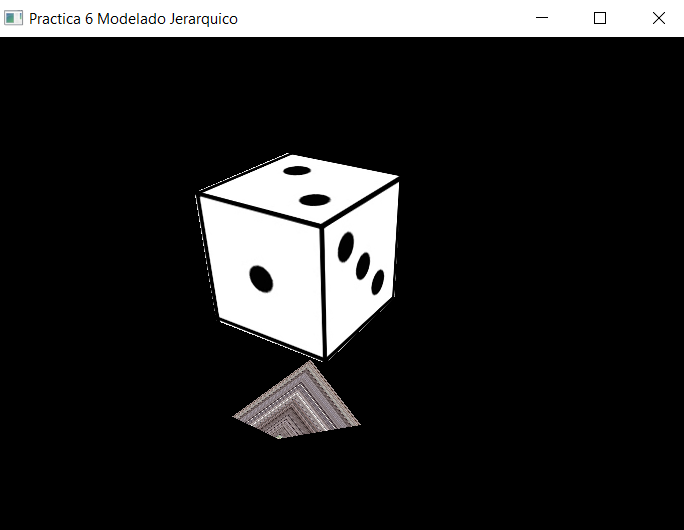
\includegraphics[scale = .6]{img/dado1.png}\\[.05cm] % Imagen1
		Figura 1\\[.65cm]
		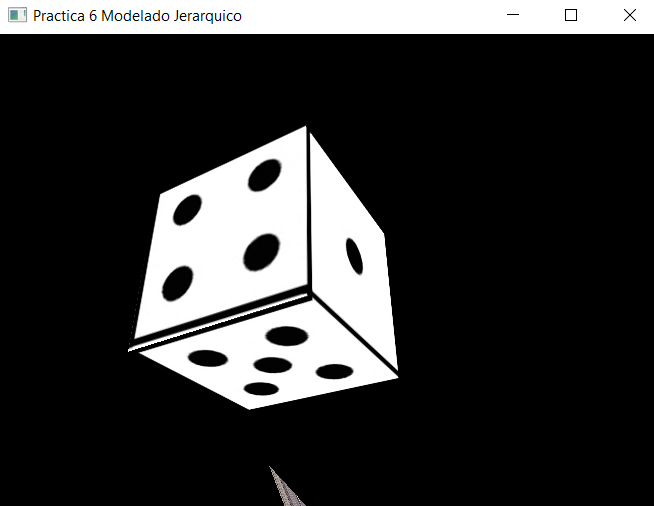
\includegraphics[scale = .6]{img/dado2.png}\\[.05cm] % Imagen1
		Figura 2\\[.65cm]

 \raggedright 
\vspace{.5cm}	
\section{Problemas presentados}
\justify
No se presentaron problemas al realizar esta práctica. \\[.4cm]

\section{Comentarios}
\justify
Fue una práctica bastante sencilla, aprendimos a añadir textura a nuestros objetos creados en openGL, para ello solamente fue necesario utilizar un software para editas la imagen (añadir canal alfa, recortar y dimensionar la imagen) y calcular las coordenadas de cada uno de los vértices del dado de nuestra imagen.\\ [.3cm]
Aprendimos a especificar que parte de la imagen queremos mostrar y en que parte queremos que se muestre.\\[.3cm]
\end{document}
